\section{Practice Problems}

\begin{frame}{Tomography}
    \begin{itemize}
        \item \textbf{Tomography} refers to \textit{imaging by section}
        \item Idea: use a penetrating wave to image sections of an object
        \item Then process those section to \textit{recreate a 3D image}
        \item Examples of tomography: X-ray, CAT scan, MRI, Ultrasound
    \end{itemize}
    \begin{center}
        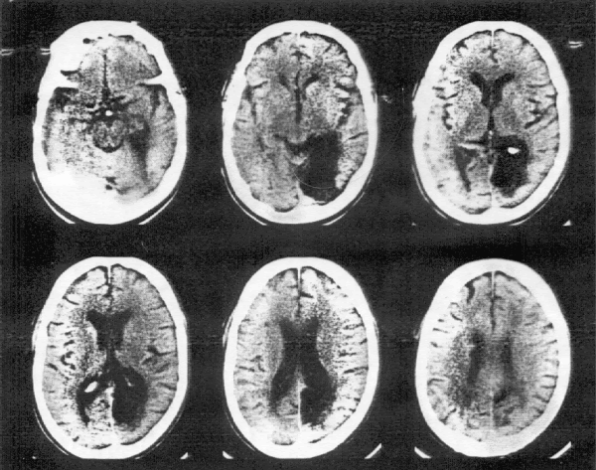
\includegraphics[width = 0.4\textwidth]{images/tomography.png}
    \end{center}
\end{frame}

\begin{frame}{Tomography}
    \textbf{Basic Tomography Example}: Suppose we have 3 types of bottles, each absorbing some amount of light: \\[1.5ex]

    \textbf{Problem}: Given an \textit{grid of bottles}, and a straight-line laser, how can we \textit{determine what bottles we have}? \\[1.5ex]
    \textbf{Idea}: Shine a light through different rows and columns and record the light absorbed. \\[1.5ex]

    \begin{center}
        \begin{tabular}{| c | c | c | c|}
            \hline &&& \\
            \textbf{Material} & Milk (M) & Juice(J) & Empty (O) \\
            \hline &&& \\
            \textbf{Light absorbed} & 3 & 2 & 1 \\
            \hline
        \end{tabular}
    \end{center}
\end{frame}

\begin{frame}{Tomography}    
    \begin{tabular}{m{0.35\textwidth} m{0.6\textwidth}}
        \multirow{2}{*}{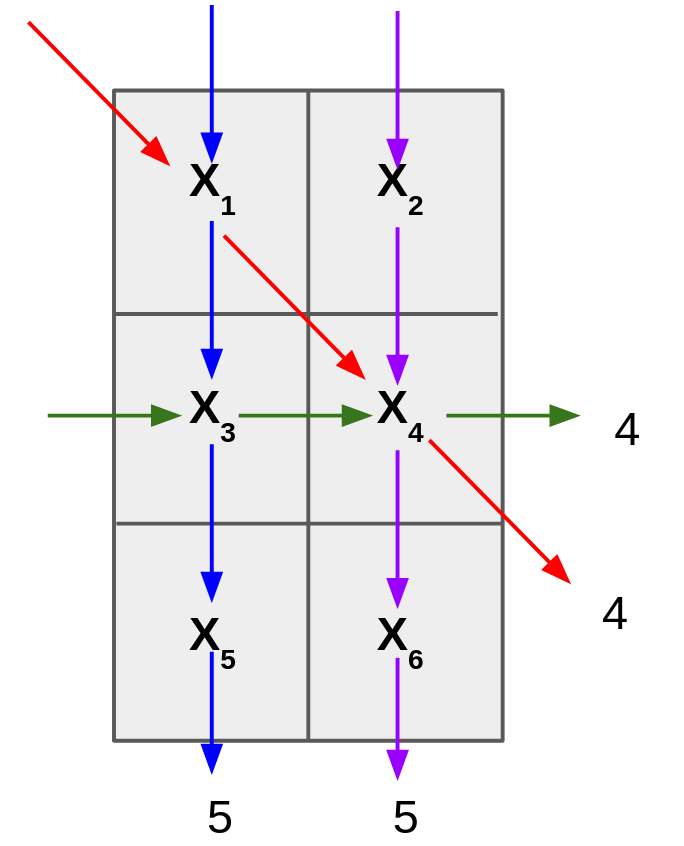
\includegraphics[width = 0.37\textwidth]{images/tomography-problem.png}} & Suppose \textbf{each bottle absorbs $X_i$ light}, and we \textit{record the light absorbed from these four light rays}. \\
        &\\[-2ex]
        & Write the \textbf{system of equations} describing the light absorbed by each bottle. \\
        &\\[-2ex]
        & Is this system \textit{solvable}? Why or why not? \\
        & What if we know each $X_i$ must be \textit{either 1, 2, or 3}?
    \end{tabular}
\end{frame}

\begin{frame}{Tomography [Solution]}
    \textcolor{blue}{
        \begin{tabular}{m{0.35\textwidth} m{0.6\textwidth}}
            \multirow{2}{*}{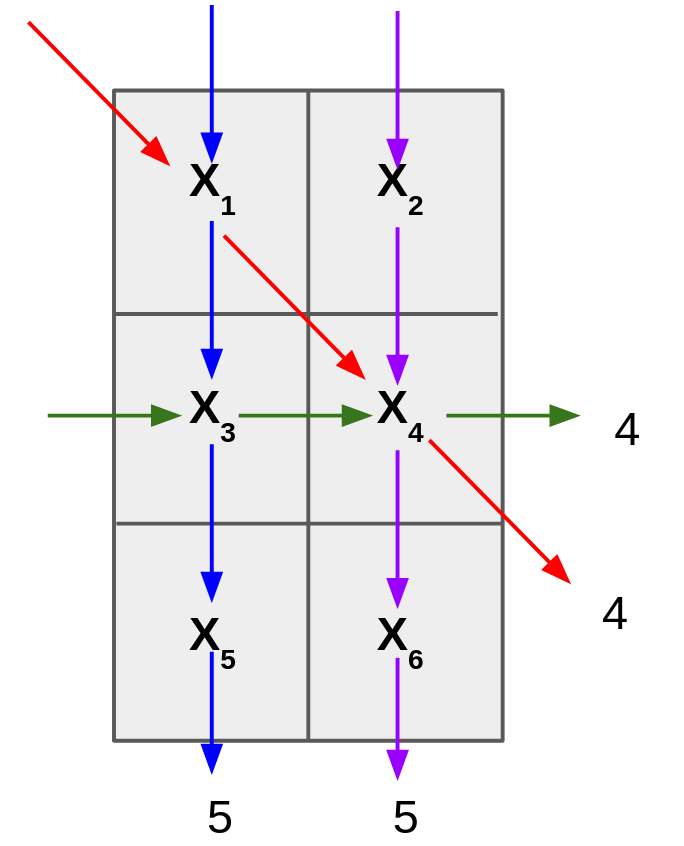
\includegraphics[width = 0.35\textwidth]{images/tomography-problem.png}} & 
            $X_1+ X_4 = 4$ \\
            & $X_1 + X_3 + X_5 = 5$ \\[-0.5ex]
            & $X_2 + X_4 + X_6 = 5$ \\[-0.5ex]
            & $X_3+ X_4 = 5$ \\
            & \quad\quad\quad\quad$\Downarrow$ \\
            & $\begin{bmatrix}[cccccc|c]
                1 & 0 & 0 & 1 & 0 & 0 & 4 \\
                1 & 0 & 1 & 0 & 1 & 0 & 5 \\
                0 & 1 & 0 & 1 & 0 & 1 & 5 \\
                0 & 0 & 1 & 1 & 0 & 0 & 5
            \end{bmatrix}$ \\
            & \quad\quad\quad\quad$\Downarrow$ \\
            & $\begin{bmatrix}[cccccc|c]
                1 & 0 & 0 & 0 & 0.5 & 0 & 2 \\
                0 & 1 & 0 & 0 & 0.5 & 1 & 3 \\
                0 & 0 & 1 & 0 & 0.5 & 0 & 3 \\
                0 & 0 & 0 & 1 & -0.5 & 0 & 2
            \end{bmatrix}$
        \end{tabular}
    }
\end{frame}

\begin{frame}{Tomography [Solution]}
    \textcolor{blue}{
        \begin{align*}
            \begin{bmatrix}[cccccc|c]
                1 & 0 & 0 & 0 & 0.5 & 0 & 2 \\
                0 & 1 & 0 & 0 & 0.5 & 1 & 3 \\
                0 & 0 & 1 & 0 & 0.5 & 0 & 3 \\
                0 & 0 & 0 & 1 & -0.5 & 0 & 2
            \end{bmatrix}
        \end{align*}
        This system would have \textbf{infinitely many solutions}, but we can solve the system because we know all $X_i$ must be 1, 2, or 3! \\[1.5ex]
        $X_1 + 0.5X_5 = 2$ \qquad $\,\,\Longrightarrow$ \quad $X_1 = 1$ and $X_5 = 2$. \\[0.5ex]
        $X_3 + 0.5X_5 = 3$ \qquad $\,\,\Longrightarrow$ \quad $X_3 = 2$ \\[0.5ex]
        $X_4 - 0.5X_5 = 2$ \qquad $\,\,\Longrightarrow$ \quad $X_4 = 3$ \\[0.5ex]
        $X_2 + 0.5X_5 + X_6 = 3$ $\,\Longrightarrow$ \quad $X_2 + X_6 = 2$ \quad $\Longrightarrow$ \quad $X_2 = X_6 = 1$
    }
\end{frame}

\begin{frame}{Bases in $\mathbb{R}^3$}
    \begin{enumerate}
        \item \textbf{True/False}: There exists a scalar $x$ such that the vectors 
        $\bigg\{
            \begin{bmatrix} 
                1 \\ 1 \\ 1 
            \end{bmatrix}, 
            \begin{bmatrix}
                1 \\ x \\ x^2
            \end{bmatrix}
        \bigg\}$ form a basis for $\mathbb{R}^3$.\\[2ex]
        \item \textbf{True/False}: There exists a scalar $x$ such that the vectors 
        $\bigg\{
            \begin{bmatrix} 
                0 \\ 1 \\ x 
            \end{bmatrix}, 
            \begin{bmatrix}
                x \\ 0 \\ 1
            \end{bmatrix},
            \begin{bmatrix}
                x \\ 1 \\ 1 + x
            \end{bmatrix}
        \bigg\}$ form a basis for $\mathbb{R}^3$.
    \end{enumerate}
\end{frame}

\begin{frame}{Bases in $\mathbb{R}^3$ [Solution]}
    \setbeamertemplate{itemize item}{\color{blue}{$\bullet$}}
    \begin{enumerate}
        \color{blue}
        \item<blue@1-> Can \textit{two vectors} ever be a basis for a \textbf{3 dimensional vector space}?
        \begin{itemize}
            \color{blue}
            \item<blue@1-> No! 
            \item<blue@1-> The two vectors considered in the question can \textbf{never} be a basis for the three dimensional vector space
        \end{itemize}
        \item<blue@1-> To form a basis for a vector space, the vectors must: \textbf{span the space} and be  \textbf{independent}.
        \begin{itemize}
            \color{blue}
            \item<blue@1-> Are the three vectors \textbf{linearly independent}?
            \item<blue@1-> No! The first two vectors sum to give the third.
            \item<blue@1-> Therefore, no matter what the value of x is, these three vectors can \textbf{never} form a basis for the vector space $\mathbb{R}^3$.
        \end{itemize}
    \end{enumerate}
\end{frame}

\begin{frame}{Spring 2015 Midterm 1: Alice's Photos}
    At the beginning of each day, Alice puts \$1 of her money into the stock market. At the end of the day she sells her stocks and looks at how much money she got back. She lets a Berkeley-based mutual fund manage the \$1 she invests. This fund invests in three companies from the area: Friendly Faces Inc., Search and Spend Inc., and Delicious Devices Inc.\\[2ex]
    Each company has a growth $g_f(i), g_(i),$ and $g_d(i)$ on dat $i$. What that means is that if Alice invests \$1 in Friendly Faces on day $i$, then she gets back $g_f(i)$ dollars at the end of day $i$. The mutual fund invests fractions $\alpha_f, \alpha_s,$ and $\alpha_d$ of Alice's money in each of the three companies. Note that these fractions are always the same (i.e. they do not change from one day to the next), and that \textbf{all of her money is always invested in the market}.
\end{frame}

\begin{frame}{Spring 2015 Midterm 1: Alice's Photos}
    \textbf{Part 1}: Using the terms defined above, write an expression using an \textbf{inner product} that would \textit{compute how many dollars Alice gets back after the first day}. 
\end{frame}

\begin{frame}{Spring 2015 Midterm 1: Alice's Photos [Solution]}
    \textcolor{blue}{
        \textbf{The model:} Let us first think about how to model the situation, before the math:
        \begin{itemize}
            \color{blue}
            \item<blue@1-> One thing that we notice is that we have \textbf{three growth functions}, each of which represent \textit{some sort of component of Alice’s investments}.  
            \item<blue@1-> Additionally, we have \textbf{investment fractions} corresponding to each of these components.  
            \item<blue@1-> Finally, we want to find the \textit{total amount of money Alice would get after one day}.  The operations needed to do this: \textbf{summing over the products of components sound awfully like an inner product}.  Additionally, it seems natural to \textit{represent the growth and the investment fraction as vectors}.  
        \end{itemize}
    }
\end{frame}

\begin{frame}{Spring 2015 Midterm 1: Alice's Photos [Solution]}
    \color{blue}{
        Growth Vector:
        \begin{align*}
            \vec{g}(1) = \begin{bmatrix}
                g_f(1) \\ g_s(1) \\ g_d(1)
            \end{bmatrix}
        \end{align*}
        Investment Vector:
        \begin{align*}
            \vec{\alpha} = \begin{bmatrix}
                \alpha_f \\ \alpha_s \\ \alpha_d
            \end{bmatrix}
        \end{align*}
        Dollars returned after Day 1:
        \begin{align*}
            \vec{g}(1)^T\vec{\alpha} = g_f(1)\alpha_f + g_s(1)\alpha_s + g_d(1)\alpha_d
        \end{align*}
    }
\end{frame}

\begin{frame}{Spring 2015 Midterm 1: Alice's Photos}
    \textbf{Part 2}: Assume that Alice gets \$1.7 back from her \$1 investment on the first day (i.e. the result of the expression you wrote in part 1 is \$1.7). \\[2ex]
    On the second day, Alice again invests \$1, but gets \$0 back! This makes Alice angry, and she wants to find out the investment strategy of the mutual fund. \\[1.5ex]
    She does some research and finds that $g_f(1) = 2, g_s(1) = 1,$ and $g_d(1) = 2$, abd on te second dat $g_f(2) = 2, g_s(2) = 2,$ but $g_d(2) = -3$. \\[1.5ex]
    Write a matrix equation Alice could use to find our what the mutual fund's investment strategy was (i.e. find the values of $\alpha_f, \alpha_s,$ and $\alpha_d$).
\end{frame}

\begin{frame}{Spring 2015 Midterm 1: Alice's Photos [Solution]}
    \begin{itemize}
        \color{blue}
        \item<blue@1-> First thing we need to note is that we are \textbf{solving for the alpha-vector}
        \item<blue@1-> We get \textbf{two equations} from noticing the following:
        \begin{align*}
            \vec{g}(1)^T \vec{\alpha} = 1.7, \vec{g}^T \vec{\alpha} = 0
        \end{align*}
        \item We have three unknowns… \textit{how do we get the third equation}?
    \end{itemize}
\end{frame}

\begin{frame}{Spring 2015 Midterm 1: Alice's Photos [Solution]}
    \begin{itemize}
        \color{blue}
        \item<blue@1-> Key idea: \textit{all of Alice’s money is invested}, so:
        \begin{align*}
            \alpha_f + \alpha_s + \alpha_d = 1
        \end{align*}
        \item<blue@1-> If we write our equations in \textbf{matrix form}:
        \begin{align*}
            \begin{bmatrix}
                2 & 1 & 2 \\
                2 & 2 & 3 \\
                1 & 1 & 1
            \end{bmatrix} 
            \begin{bmatrix}
                \alpha_f \\ \alpha_s \\ \alpha_d
            \end{bmatrix} = 
            \begin{bmatrix}
                1.7 \\ 0 \\ 1
            \end{bmatrix}
        \end{align*}
        \item<blue@1-> Assuming the matrix is invertible (it is)
        \begin{align*}
            \begin{bmatrix}
                \alpha_f \\ \alpha_s \\ \alpha_d
            \end{bmatrix} = 
            \begin{bmatrix}
                2 & 1 & 2 \\
                2 & 2 & 3 \\
                1 & 1 & 1
            \end{bmatrix}^{-1}
            \begin{bmatrix}
                1.7 \\ 0 \\ 1
            \end{bmatrix}
        \end{align*}
    \end{itemize}
\end{frame}

\begin{frame}{Page Rank}
    \small{
        \begin{center}
            \begin{tikzpicture}[shorten >=1pt,node distance=0.5cm]
                \node[state, draw=none] (hidden) {};
                \node[state, left=of hidden, align=center] (fs) {Food \\[-1ex] Store-\\[-1ex]room};
                \node[state, right=of hidden, align=center] (sr) {Sleep \\[-1ex] Room};
                \node[state, below=of hidden, align=center] (pr) {Play \\[-1ex] Room};
                \draw[every loop]
                    (fs) edge[loop left] node{0.5} (fs)
                    (sr) edge[loop right] node{0.5} (sr)
                    (pr) edge[loop left] node{$p_3$} (pr)
                    (fs) edge[bend left, auto=left] node{0.5} (sr)
                    (sr) edge[auto=right] node{0.4} (fs)
                    (pr) edge[auto=right]  node{$p_1$}(fs)
                    (sr) edge[auto=right] node{0.1} (pr)
                    (pr) edge[auto=right, bend right] node{$p_2$} (sr);
            \end{tikzpicture}
        \end{center}
        (a) Let the number of furballs in each room (Food Storeroom, Sleep Room, and Play Room) at time $n$ be $x_f[n]$, $x_s[n]$, and $x_p[n]$, respectively. We would like to find the \textbf{transition matrix} $A$ such that 
        \begin{align*}
            \begin{bmatrix}
                x_f[n + 1] \\
                x_s[n + 1] \\
                x_p[n + 1]
            \end{bmatrix} = A
            \begin{bmatrix}
                x_f[n] \\
                x_s[n] \\
                x_p[n]
            \end{bmatrix}
        \end{align*}
        Write $A$ using the numbers and variables in the diagram.
    }
\end{frame}

\begin{frame}{Page Rank [Solution]}
    \color{blue}{
        The \textbf{transition matrix} is
        \begin{align*}
            A = \begin{bmatrix}
                0.5 & 0.4 & p_1 \\
                0.5 & 0.5 & p_2 \\
                0 & 0.1 & p_3
            \end{bmatrix}
        \end{align*}
        Remember that the element at row $i$, column $j$ represents the number of furballs going from room $j$ to room $i$.
    }
\end{frame}

\begin{frame}{Page Rank}
    (b) We know that \textit{no furballs enter or leave} the configuration of tunnels shown above and that during the time you're observing the behavior, \textit{no furballs die or are born}. What \textbf{constraint} does this place on the values of $p_1, p_2, p_3$? Write your answer in \textit{equation form}.
\end{frame}

\begin{frame}{Page Rank [Solution]}
    (b) We know that \textit{no furballs enter or leave} the configuration of tunnels shown above and that during the time you're observing the behavior, \textit{no furballs die or are born}. What \textbf{constraint} does this place on the values of $p_1, p_2, p_3$? Write your answer in \textit{equation form}.\\[2ex]
    \color{blue}{
        No furballs enter or leave the system, so the \textbf{sum of each column must be 1}. So,
        \begin{align*}
            p_1 + p_2 + p_3 = 1
        \end{align*}
    }
\end{frame}

\begin{frame}{Page Rank}
    (c) Suppose we let $\vec{p} = \begin{bmatrix}
        p_1 \\ p_2 \\ p_3
    \end{bmatrix}$ and $\vec{x}[n] = \begin{bmatrix}
        x_f[n] \\ x_s[n] \\ x_p[n]
    \end{bmatrix}$, and that we are sure that $x_p[n]$ is nonzero. \\[2ex]
    Express $\vec{p}$ as a function of the numbers in the diagram. $\vec{x}[n]$, and $\vec{x}[n + 1]$. (\textit{Hint: what is the relationship between $\vec{x}[n + 1]$ and $\vec{x}[n]$?})
\end{frame}

\begin{frame}{Page Rank [Solution]}
    (c) Suppose we let $\vec{p} = \begin{bmatrix}
        p_1 \\ p_2 \\ p_3
    \end{bmatrix}$ and $\vec{x}[n] = \begin{bmatrix}
        x_f[n] \\ x_s[n] \\ x_p[n]
    \end{bmatrix}$, and that we are sure that $x_p[n]$ is nonzero. \\[2ex]
    Express $\vec{p}$ as a function of the numbers in the diagram. $\vec{x}[n]$, and $\vec{x}[n + 1]$. (\textit{Hint: what is the relationship between $\vec{x}[n + 1]$ and $\vec{x}[n]$?})

    \color{blue}{
        \begin{align*}
            \vec{p} = \frac{1}{x_p[n]} \Bigg(\vec{x}[n + 1] - x_f[n]
            \begin{bmatrix}
                0.5 \\ 0.5 \\ 0
            \end{bmatrix} - x_s[n]
            \begin{bmatrix}
                0.4 \\ 0.5 \\ 0.1
            \end{bmatrix}\Bigg)
        \end{align*}
    }
\end{frame}

\begin{frame}{Steady State}
    (a) Consider a 2x2 matrix $A$, where max(eigenvalues($A$)) $>$ 1. Is it possible for the system defined by $x(t + 1) = Ax(t)$ to be \textbf{stable} (i.e. non-exploding) for some initial $x$?
\end{frame}

\begin{frame}{Steady State [Solution]}
    (a) Consider a 2x2 matrix $A$, where max(eigenvalues($A$)) $>$ 1. Is it possible for the system defined by $x(t + 1) = Ax(t)$ to be \textbf{stable} (i.e. non-exploding) for some initial $x$? \\[2ex]

    \color{blue}{
        Yes, but only as long as there is \textbf{another eigenvalue such that abs(eigenvalue) $\leq$ 1}  and only for an \textbf{appropriate initial state $x_0$}
    }
\end{frame}

\begin{frame}{Steady State}
    (b) Given a \textbf{conservative} state transition matrix $A$, is it possible for $A$ to have \textbf{multiple eigenvectors} corresponding to the eigenvalue 1? \textit{What does it say about the system?}
\end{frame}

\begin{frame}{Steady State [Solution]}
    (b) Given a \textbf{conservative} state transition matrix $A$, is it possible for $A$ to have \textbf{multiple eigenvectors} corresponding to the eigenvalue 1? \textit{What does it say about the system?} \\[2ex]
    \color{blue}{
        Yes. There is a set of \textbf{linearly independent steady-state}s, and \textit{any linear combination of those states is stable}.
    }
\end{frame}
